\section{Studio della scia del profilo alare Naca 0015}
La presente esercitazione si pone come obiettivo lo studio della scia del profilo alare NACA 0015 al variarre dell'incidenza e del numero di Reynolds. In particolare si vuole:
\begin{itemize}
    \item Valutare e diagrammare il coefficiente di resistenza aerodinamica $c_D(\alpha, Re)$;
    \item Valutare e diagrammare la distribuzione della velocità nella scia e della sua dimensione trasversale al variare dell'incidenza e del numero di Reynolds.
\end{itemize}

\subsection{Descrizione dell'esperimento}
La scia contiene informazioni legate ai processi dissipativi di energia cinetica, da tali informazioni è possibile risalire alla forza che il profilo esercita sul flusso.\\\\
Per misurare il coefficiente di resistenza, risulta comodo applicare il teorema della variazione della quantità di moto. Tale teorema stabilisce che definito un volume di controllo arbitrario attorno al corpo, la variazione della quantità di moto $\vec Q$ nell'unità di tempo subita dalla corrente nell'attraversare il volume è pari alla risultante delle forze che agiscono sul volume di controllo.
\begin{equation*}
    \frac{d\vec Q}{dt} = \vec{F}
\end{equation*}
Le forze applicate al volume possono agire attraverso il contorno esterno al volume e/o dall'interno del volume stesso, ovvero attraverso il corpo che applica una sua forza. Nella figura il volume di controllo è rappresentato dalla linea tratteggiata che circonda esternamente il volume e contorna il corpo immerso nel volume.
\begin{figure}[H]
    \centering
    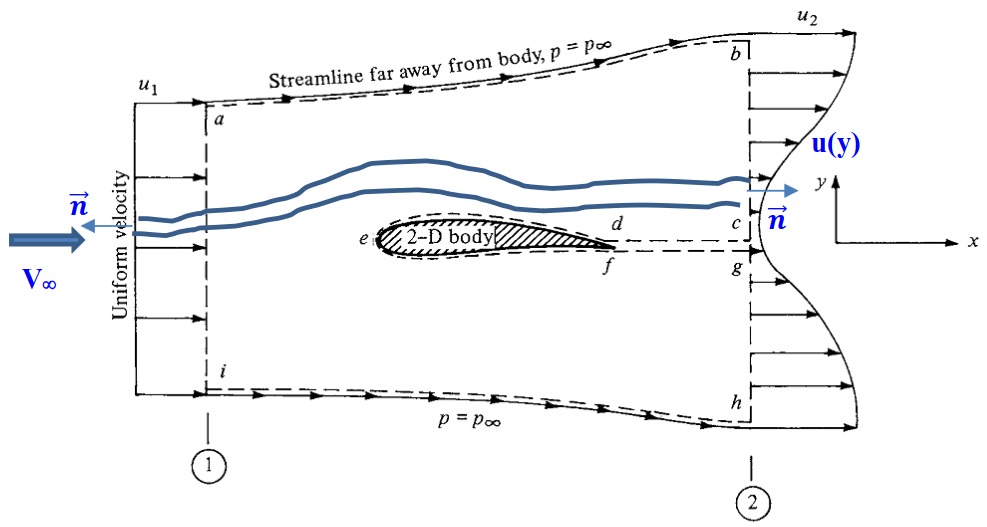
\includegraphics[width=.8\textwidth]{images/6/thqdm.png}
\end{figure}

\noindent Applicando il teorema della quantità di moto nella direzione della velocità a monte $V_\infty$, si ricava dunque la resistenza aerodinamica $D$:
\begin{equation*}
    D = \frac{\Delta Q}{\Delta t}
\end{equation*}
La quantità di moto, per definizione risulta essere $Q=mV=(\rho AL )V$. La derivata della massa nel tempo rappresenta la portata in massa. Pertanto:
\begin{equation*}
    \frac{dm}{dt} = \dot m = \rho A u \quad \Rightarrow \quad D= \dot m \Delta V
\end{equation*}
La forza di resistenza al moto elementare si scrive come:
\begin{equation*}
    dD = d\dot m \Delta V
\end{equation*}
La portata elementare è $d\dot m = \rho u dA$, ma considerando profondità unitaria questa può essere espressa come $d\dot m = \rho u dy$.\\\\
La variazione di velocità lungo una linea di corrente risulta essere:
\begin{equation*}
    \Delta V = V_\infty - u
\end{equation*}
Dove $V_\infty$ rappresenta la velocità a monte e $u$ la velocità a valle, variabile lungo $y$.\\\\
Sostituendo la variazione di velocità nella relazione per la resistenza aerodinamica elementare si ottiene:
\begin{equation*}
    dD = \rho u (V_\infty -u ) dy
\end{equation*}
Si può quindi valutare la resistenza aerodinamica integrando tale relazione:
\begin{equation*}
    D = \int_{-\infty}^\infty dD = \rho \int_{-\infty}^\infty u (V_\infty - u) dy
\end{equation*}
Introducendo il coefficiente di resistenza aerodinamica del profilo alare, rispetto ad una superifice di profondità unitaria ($S = c\cdot1$):
\begin{equation*}
    c_D = \frac{D}{\frac12 \rho V_\infty^2 c}
\end{equation*}
Si ricava quindi:
\begin{equation*}
    c_D = \frac 2c \int_{-\infty}^\infty \frac {u}{V_\infty} \left( 1-\frac{u}{V_\infty}\right) dy
\end{equation*}
Per calcolare la distribuzione di velocità normalizzata $u/V_\infty$, che risulta essere funzione di $y$, si scrive l'equazione di Bernoulli:
\begin{equation*}
    \begin{split}
        &\text{A monte } p_{0\infty} - p_\infty = \frac 12 \rho V_\infty^2\\
        &\text{Nella scia } p_{0} - p = \frac 12 \rho u^2
    \end{split}
\end{equation*}
Da queste equazioni si ricava:
\begin{equation*}
    \frac{u}{V_\infty} = \sqrt{\frac{p_0 - p}{p_{0\infty} - p_\infty}}
\end{equation*}
Si può quindi riscrivere la relazione per il coefficiente di resistenza come:
\begin{equation*}
    c_D = \frac 2c \int_{-\infty}^{\infty} \left( \sqrt{\frac{p_0 - p}{p_{0\infty} - p_\infty}} - \frac{p_0 - p}{p_{0\infty} - p_\infty} \right) dy
\end{equation*}

\subsection{Catena di misura}
La catena di misura è la stessa descritta nell'esercitazione precedente. Il profilo alare è posizionato in una galleria del vento aperta, ma questa volta anziché rilevare i dati dalle prese di pressione statica sulla superficie del profilo, si misura la pressione totale nella scia, mediante un rake di prese di pressione totale $p_0(y)$.
\begin{figure}[H]
    \centering
    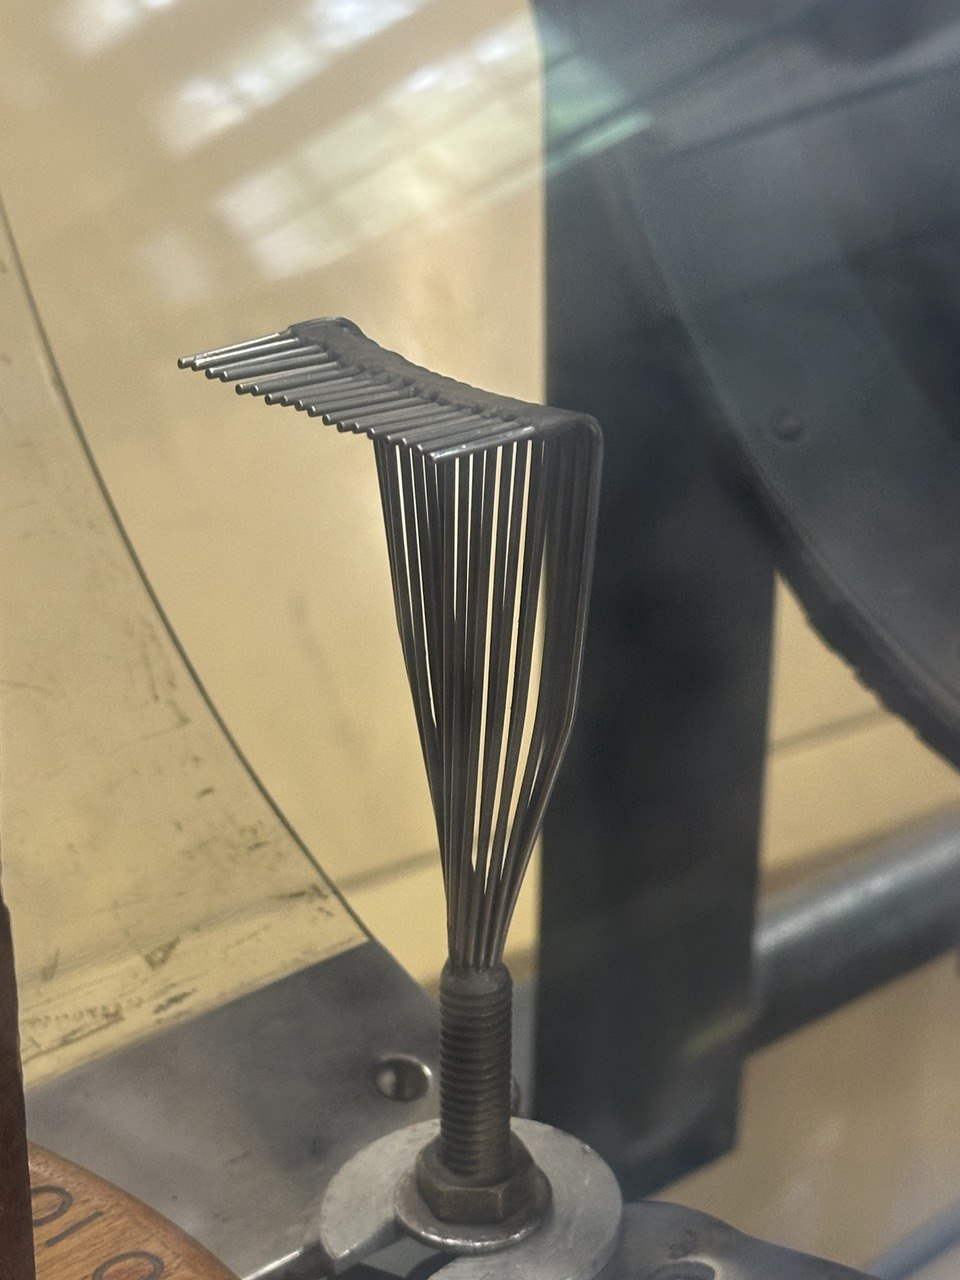
\includegraphics[width=.7\textwidth]{images/6/rake.jpg}
    \caption{Rake di prese di pressione sulla scia}
\end{figure}

\noindent In particolare, il rack comprende 18 prese di pressione totale, distanti tra loro $\Delta y= 2mm$. Queste, assieme alle prese di pressione statica e pressione totale all'entrate della camera di prova, sono connesse ad un multimanometro differenziale, che utilizza come fluido manometrico dell'alcool etilico.

\subsection{Procedura sperimentale}\label{istogrammiscia}
Per ogni incidenza sono misurate le altezze del fluido manometrico $h_i$ oltre alle grandezze $h_{0\infty}$ e $h_\infty$ corrispondenti alle pressioni $p_{0\infty}$ e $p_0$, analogamente all'indagine precedente.\\\\
Ricordando l'espressione ricavata per il coefficiente di resistenza:
\begin{equation*}
    c_D = \frac 2c \int_{-\infty}^{\infty} \left( \sqrt{\frac{p_0 - p}{p_{0\infty} - p_\infty}} - \frac{p_0 - p}{p_{0\infty} - p_\infty} \right) dy
\end{equation*}
Utilizzando la legge di Stevino $\Delta p = \gamma_{fm} \Delta h$ e uguagliando la pressione statica a monte e la pressione statica nella scia $p_{\infty}=p$, si ottiene una relazione che lega il coefficiente di resistenza aerodinamica alle altezze rilevate dalle canne manometriche:
\begin{equation*}
    c_D = \frac 2c \int_{-\infty}^\infty \left( \sqrt{\frac{h_\infty - h_0}{h_\infty - h_{0\infty}}} - \frac{h_\infty - h_0}{h_\infty - h_{0\infty}} \right) dy 
\end{equation*}
Si ottengono quindi i seguenti istogrammi, rappresentativi delle altezze del fluido manometrico nelle varie canne del multimanometro differenziale. La prima e la seconda colonna rappresentano la pressione statica e la pressione totale a monte, mentre le altre 18 colonne rappresentano le 18 prese di pressione totale della scia.
\begin{figure}[H]
    \centering
    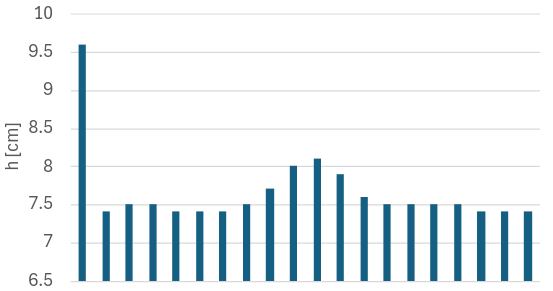
\includegraphics[width=.49\textwidth]{images/6/s1a0.png}
    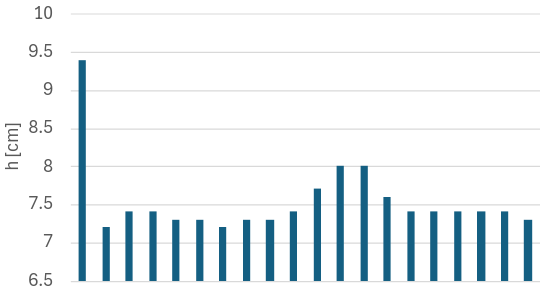
\includegraphics[width=.49\textwidth]{images/6/s1a2.png}
    \caption{Squadra 1 incidenza 0 e 2 gradi}
\end{figure}
\begin{figure}[H]
    \centering
    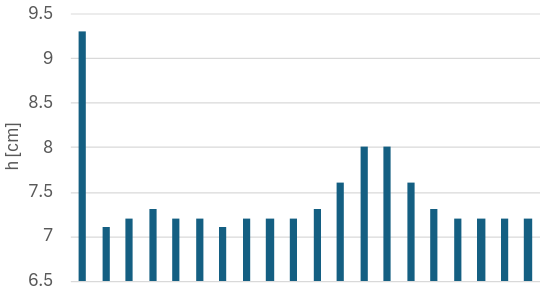
\includegraphics[width=.49\textwidth]{images/6/s1a4.png}
    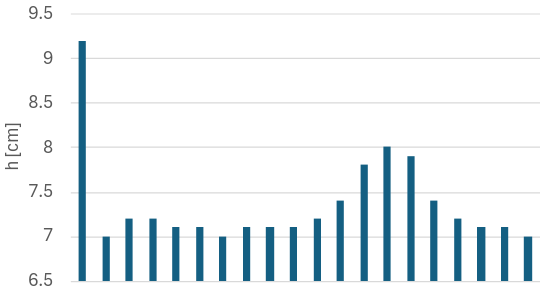
\includegraphics[width=.49\textwidth]{images/6/s1a6.png}
    \caption{Squadra 1 incidenza 4 e 6 gradi}
\end{figure}
\begin{figure}[H]
    \centering
    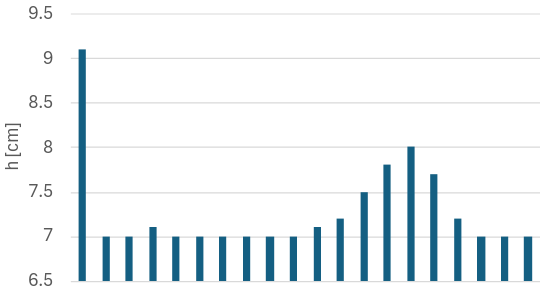
\includegraphics[width=.49\textwidth]{images/6/s1a8.png}
    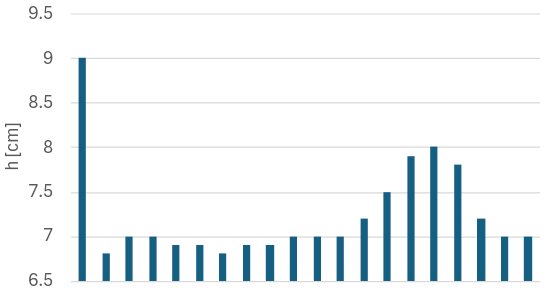
\includegraphics[width=.49\textwidth]{images/6/s1a10.png}
    \caption{Squadra 1 incidenza 8 e 10 gradi}
\end{figure}
\begin{figure}[H]
    \centering
    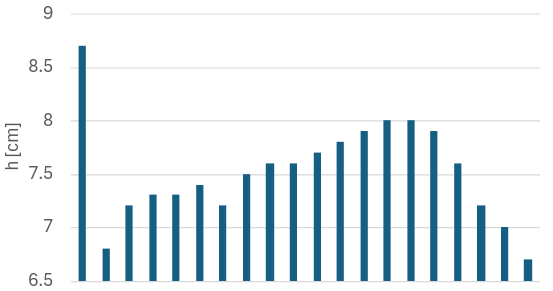
\includegraphics[width=.49\textwidth]{images/6/s1a12.png}
    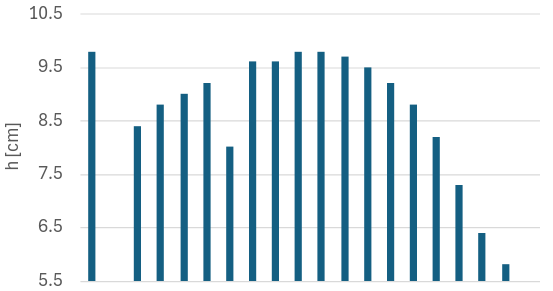
\includegraphics[width=.49\textwidth]{images/6/s2a15.png}
    \caption{Squadra 1 incidenza 12 gradi e squadra 2 incidenza 15 gradi}
\end{figure}
\begin{figure}[H]
    \centering
    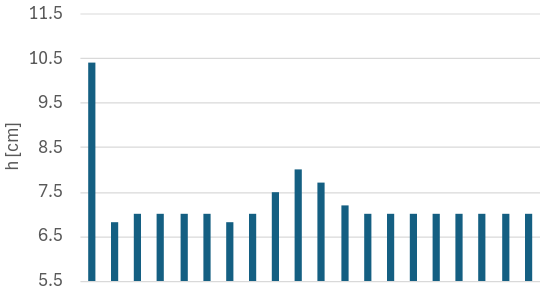
\includegraphics[width=.49\textwidth]{images/6/s2a0.png}
    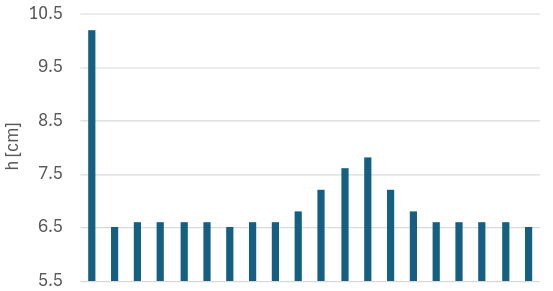
\includegraphics[width=.49\textwidth]{images/6/s2a2.png}
    \caption{Squadra 2 incidenza 0 e 2 gradi}
\end{figure}
\begin{figure}[H]
    \centering
    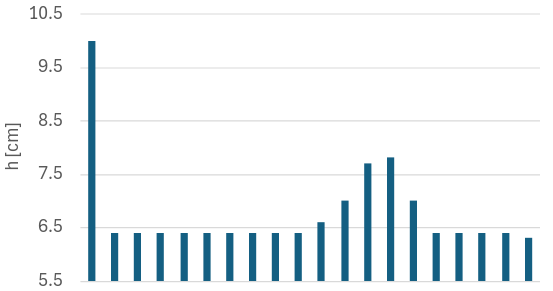
\includegraphics[width=.49\textwidth]{images/6/s2a4.png}
    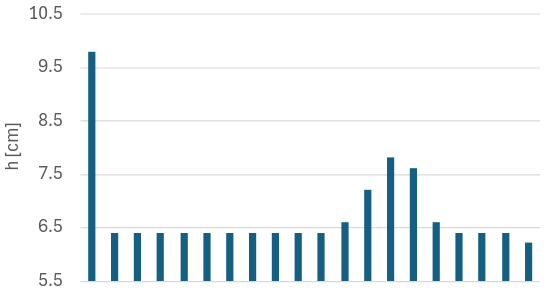
\includegraphics[width=.49\textwidth]{images/6/s2a6.png}
    \caption{Squadra 2 incidenza 4 e 6 gradi}
\end{figure}
\begin{figure}[H]
    \centering
    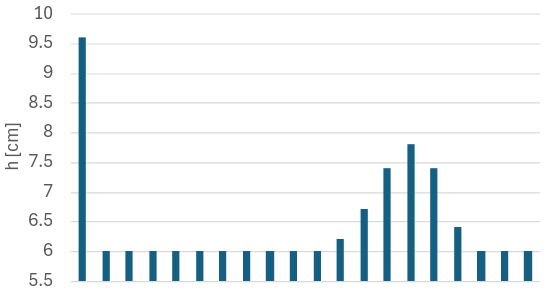
\includegraphics[width=.49\textwidth]{images/6/s2a8.png}
    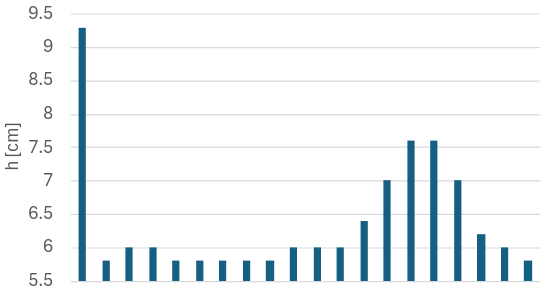
\includegraphics[width=.49\textwidth]{images/6/s2a10.png}
    \caption{Squadra 2 incidenza 8 e 10 gradi}
\end{figure}
\begin{figure}[H]
    \centering
    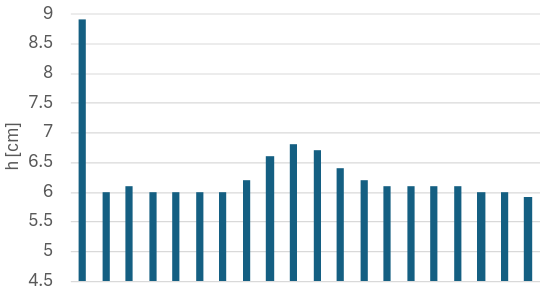
\includegraphics[width=.49\textwidth]{images/6/s3a0.png}
    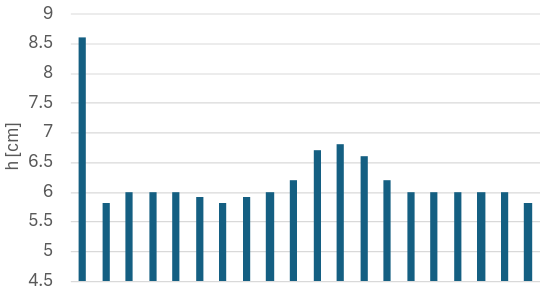
\includegraphics[width=.49\textwidth]{images/6/s3a2.png}
    \caption{Squadra 3 incidenza 0 e 2 gradi}
\end{figure}
\begin{figure}[H]
    \centering
    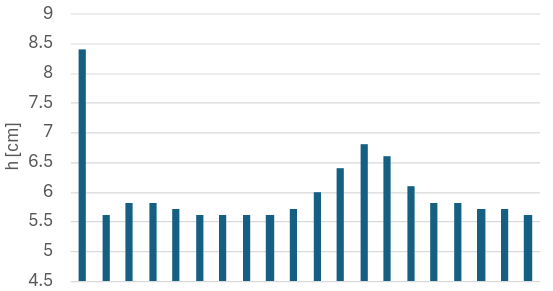
\includegraphics[width=.49\textwidth]{images/6/s3a4.png}
    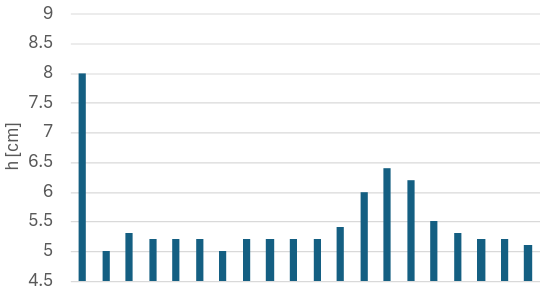
\includegraphics[width=.49\textwidth]{images/6/s3a6.png}
    \caption{Squadra 3 incidenza 4 e 6 gradi}
\end{figure}
\begin{figure}[H]
    \centering
    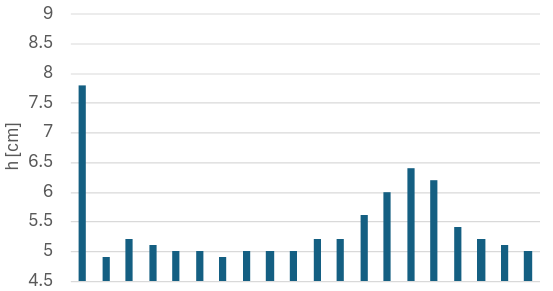
\includegraphics[width=.49\textwidth]{images/6/s3a8.png}
    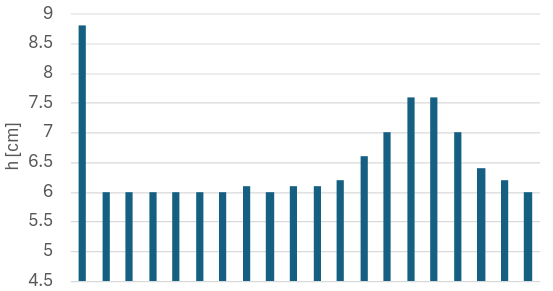
\includegraphics[width=.49\textwidth]{images/6/s3a10.png}
    \caption{Squadra 3 incidenza 8 e 10 gradi}
\end{figure}
\begin{figure}[H]
    \centering
    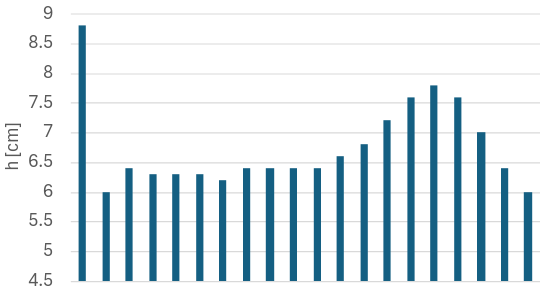
\includegraphics[width=.49\textwidth]{images/6/s3a12.png}
    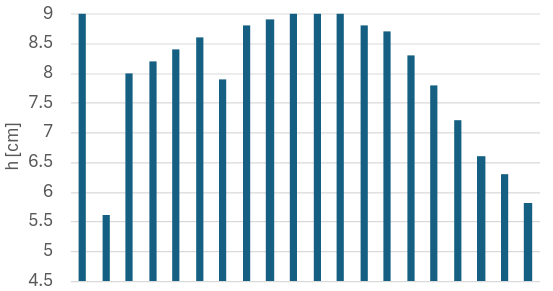
\includegraphics[width=.49\textwidth]{images/6/s3a15.png}
    \caption{Squadra 3 incidenza 12 e 15 gradi}
\end{figure}
\begin{figure}[H]
    \centering
    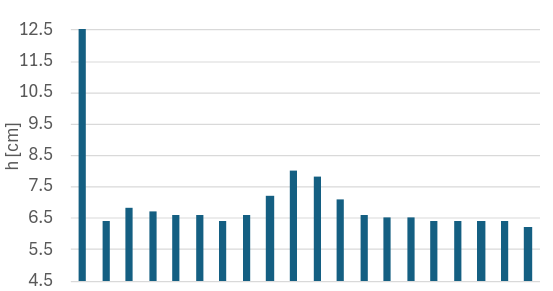
\includegraphics[width=.49\textwidth]{images/6/s4a0.png}
    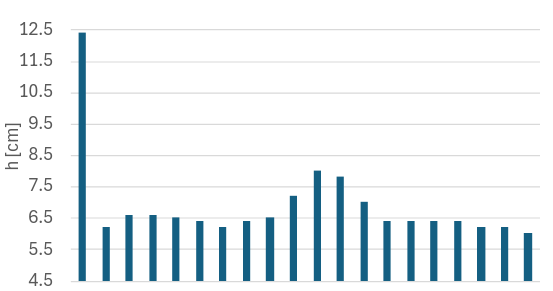
\includegraphics[width=.49\textwidth]{images/6/s4a2.png}
    \caption{Squadra 4 incidenza 0 e 2 gradi}
\end{figure}
\begin{figure}[H]
    \centering
    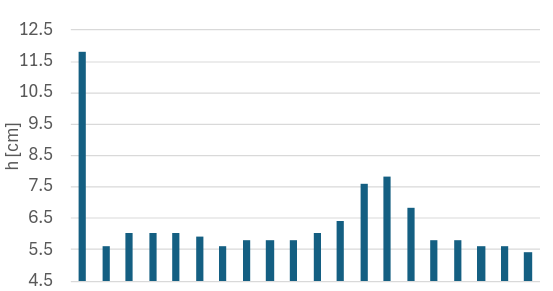
\includegraphics[width=.49\textwidth]{images/6/s4a4.png}
    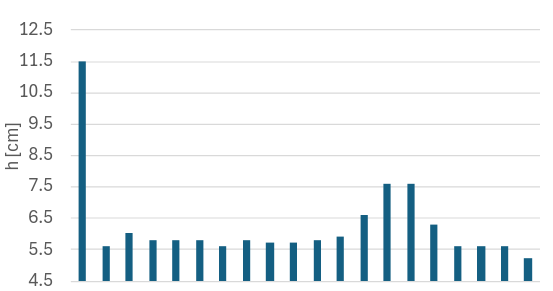
\includegraphics[width=.49\textwidth]{images/6/s4a6.png}
    \caption{Squadra 4 incidenza 4 e 6 gradi}
\end{figure}
\begin{figure}[H]
    \centering
    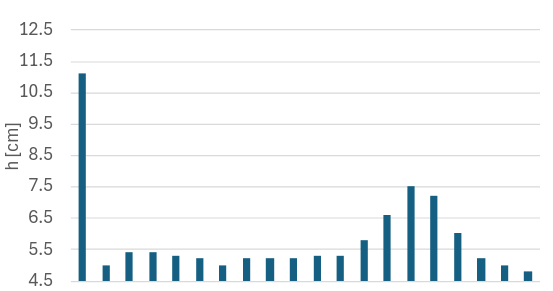
\includegraphics[width=.49\textwidth]{images/6/s4a10.png}
    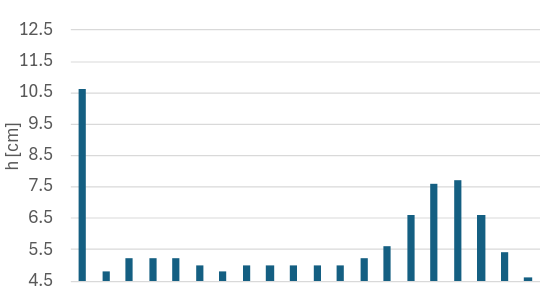
\includegraphics[width=.49\textwidth]{images/6/s4a12.png}
    \caption{Squadra 4 incidenza 10 e 12 gradi}
\end{figure}
\begin{figure}[H]
    \centering
    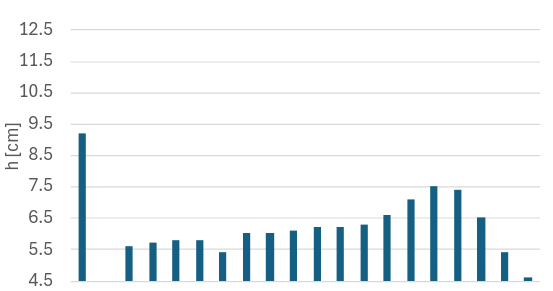
\includegraphics[width=.49\textwidth]{images/6/s4a15.png}
    \caption{Squadra 4 incidenza 15 gradi}
\end{figure}

\noindent Si osserva immediatamente dai dati grezzi come la posizione della scia si sposti verso il basso con l'aumentare dell'incidenza.

\subsection{Analisi dati}
L'analisi dati per la presente attività è condotta con l'ausilio di un codice Python, riportato in appendice \ref{b6}, e di un semplice foglio di calcolo Excel.\\\\
A partire dai dati grezzi sulle altezze delle canne manometriche, è immediato calcolare le distribuzioni di velocità, utilizzando le equazioni di Stevino e Bernoulli:
\begin{equation*}
    \frac{u(y)}{V_\infty} = \sqrt{\frac{q(y)}{q_\infty}} =  \sqrt{\frac{p_0 - p_\infty}{p_{0\infty} - p_\infty}} = \sqrt{\frac{h_\infty - h_0}{h_{\infty} - h_{0\infty}}} 
\end{equation*}
Si ottengono i seguenti diagrammi per le distribuzioni di velocità per le quattro squadre:
\begin{figure}[H]
    \centering
    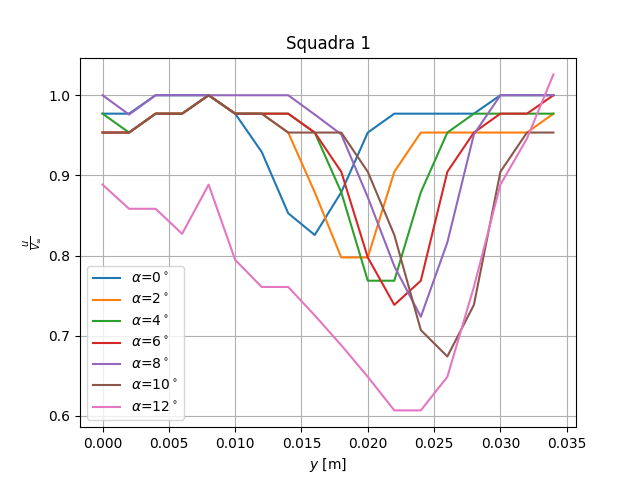
\includegraphics[width=.8\textwidth]{images/6/v1.png}
\end{figure}
\begin{figure}[H]
    \centering
    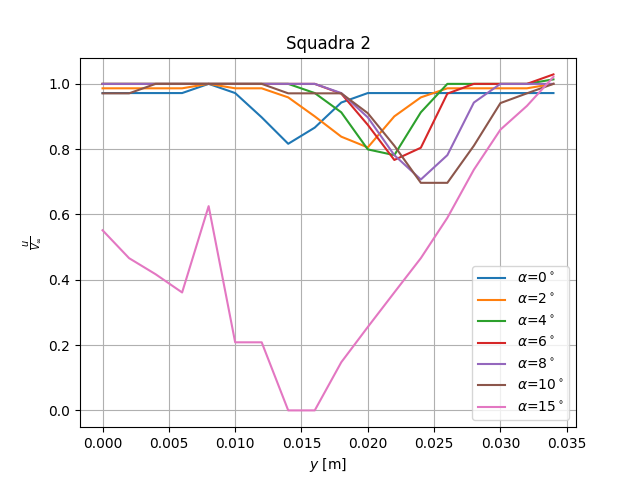
\includegraphics[width=.65\textwidth]{images/6/v2.png}
    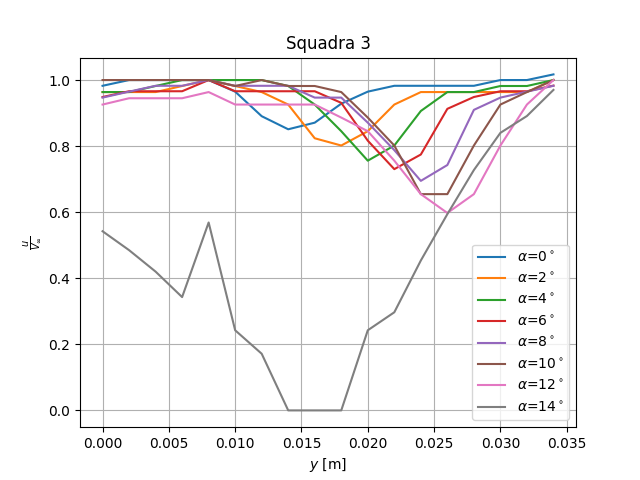
\includegraphics[width=.65\textwidth]{images/6/v3.png}
    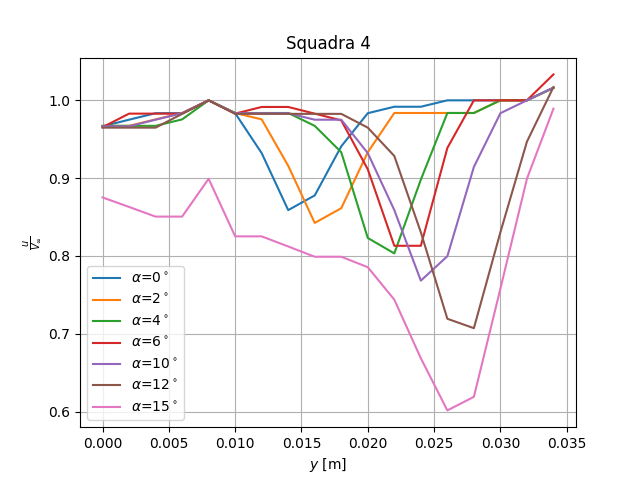
\includegraphics[width=.65\textwidth]{images/6/v4.png}
\end{figure}

\noindent Come già accennato in precedenza, si nota come la scia si sposta verso il basso ($y$ maggiori) con l'aumentare dell'incidenza $\alpha$, questo è dovuto all'effetto downwash. Inoltre, dalla distribuzione delle velocità, si osserva come all'aumentare dell'incidenza aumenti leggermente anche la dimensione trasversale della scia, finché non si arriva ad un angolo di incidenza nella condizione di stallo, in cui il flusso separa e la curva che caratterizza la distribuzione di velocità relativa a tale angolo si discosta drasticamente dalle altre.
\subsubsection{Dimensione trasversale della scia}
Si può considerare convenzionalmente la dimensione trasversale della scia $\Delta_w(\alpha)$ come il doppio della distanza tra il punto di minima velocità ed il punto dove la velocità raggiunge il 90\% della velocità all'esterno della scia.
\begin{equation*}
    \Delta_w(\alpha) = 2 (y_{u=0.9U_e} - y_{u_{min}})
\end{equation*}
\begin{figure}[H]
    \centering
    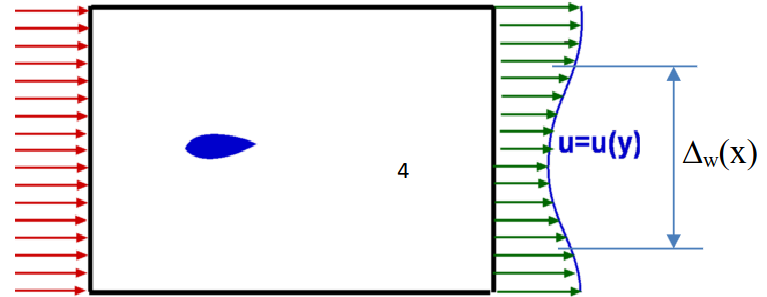
\includegraphics[width=.55\textwidth]{images/6/deltawimage.png}
\end{figure}

\noindent Utilizzando i dati ottenuti sulle distribuzioni di velocità, si ottiene il seguente diagramma per le quattro squadre:
\begin{figure}[H]
    \centering
    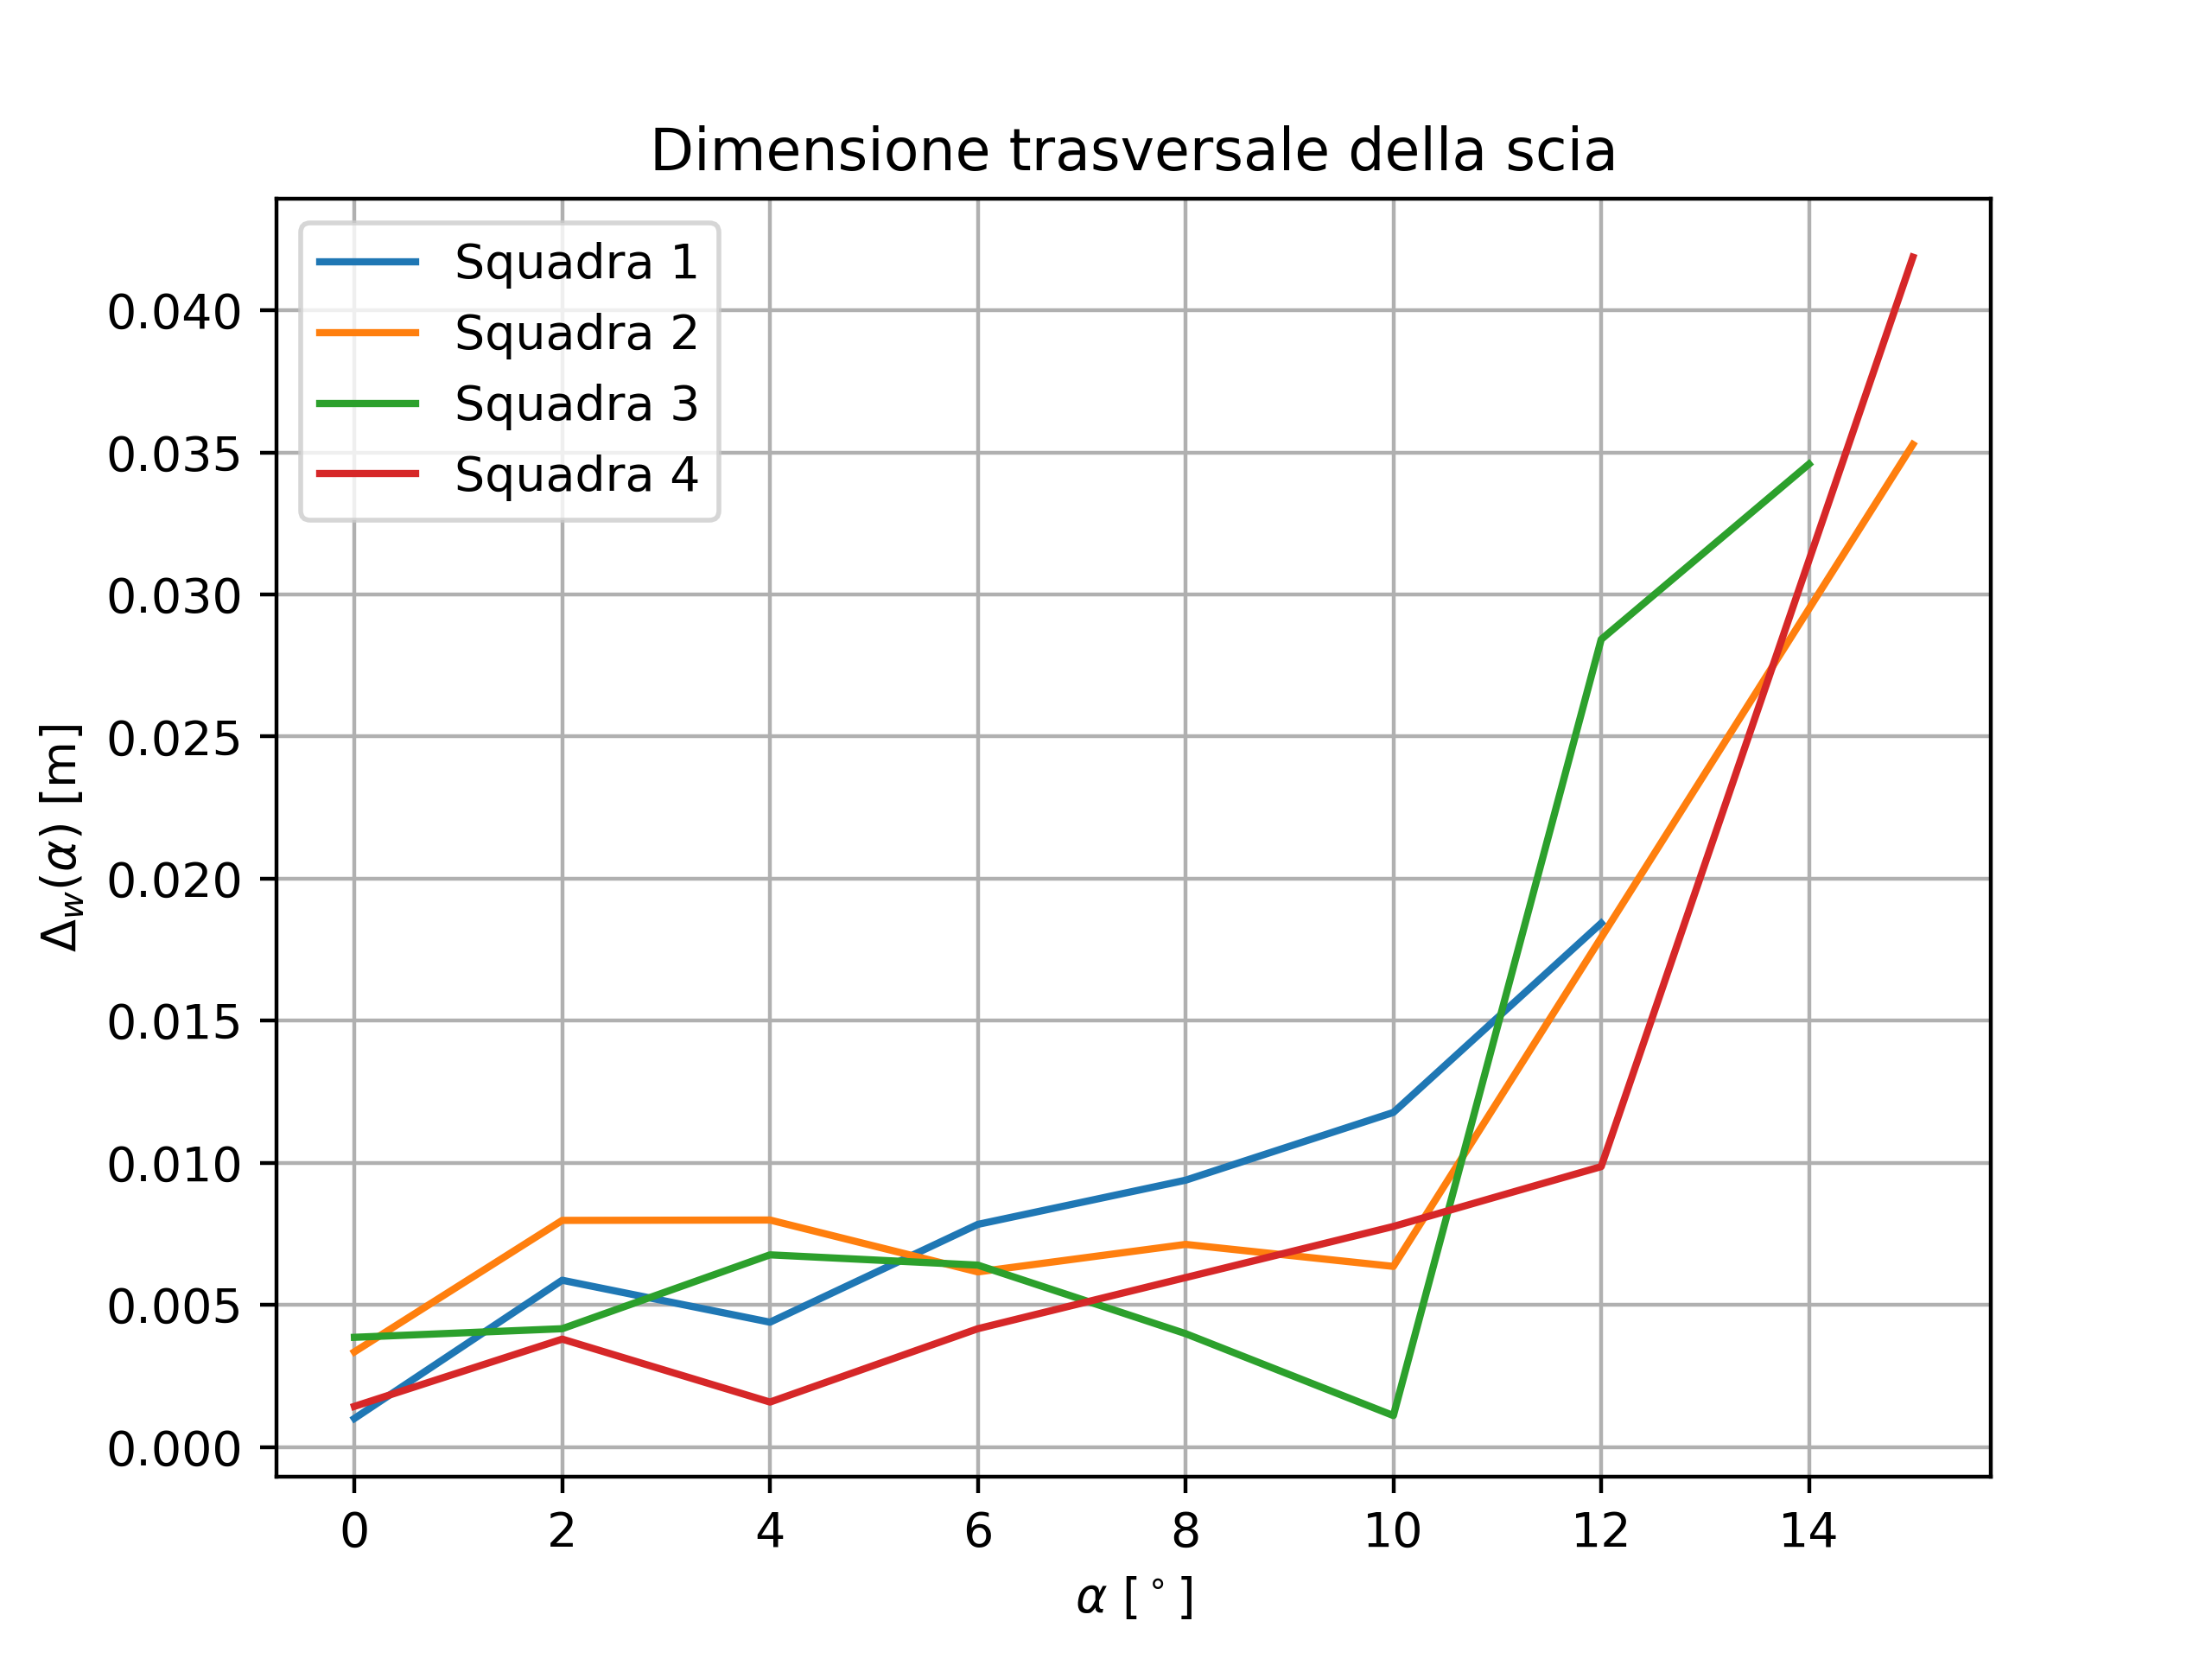
\includegraphics[width=.75\textwidth]{images/6/dim scia.png}
    \caption{Dimensione della scia al variare dell'incidenza}
\end{figure}

\noindent Si osserva come la dimensione della scia aumenti con l'incidenza, fino a subire un drastico aumento in corrispondenza della condizione di stallo.
\subsubsection{Coefficiente di resistenza aerodinamica}
Dai valori ottenuti sulle distribuzioni di velocità, si ricava il coefficiente di resistenza aerodinamica in funzione dell'incidenza:
\begin{equation*}
    c_D(\alpha) = \frac 2c \int_{-\infty}^\infty \frac{u(y)}{V_\infty}\left(1-\frac{u(y)}{V_\infty}\right)dy
\end{equation*}
Questo integrale è approssimato con la regola dei trapezi:
\begin{equation*}
    \int_a^b f(x)dx \approx \sum_{k=1}^n \frac{f(x_{k-1}) + f(x_k)}2 \Delta x_k \quad \text{con } \Delta x_k = x_k - x_{k-1}
\end{equation*}
Si ottiene quindi il seguente diagramma per le quattro squadre:
\begin{figure}[H]
    \centering
    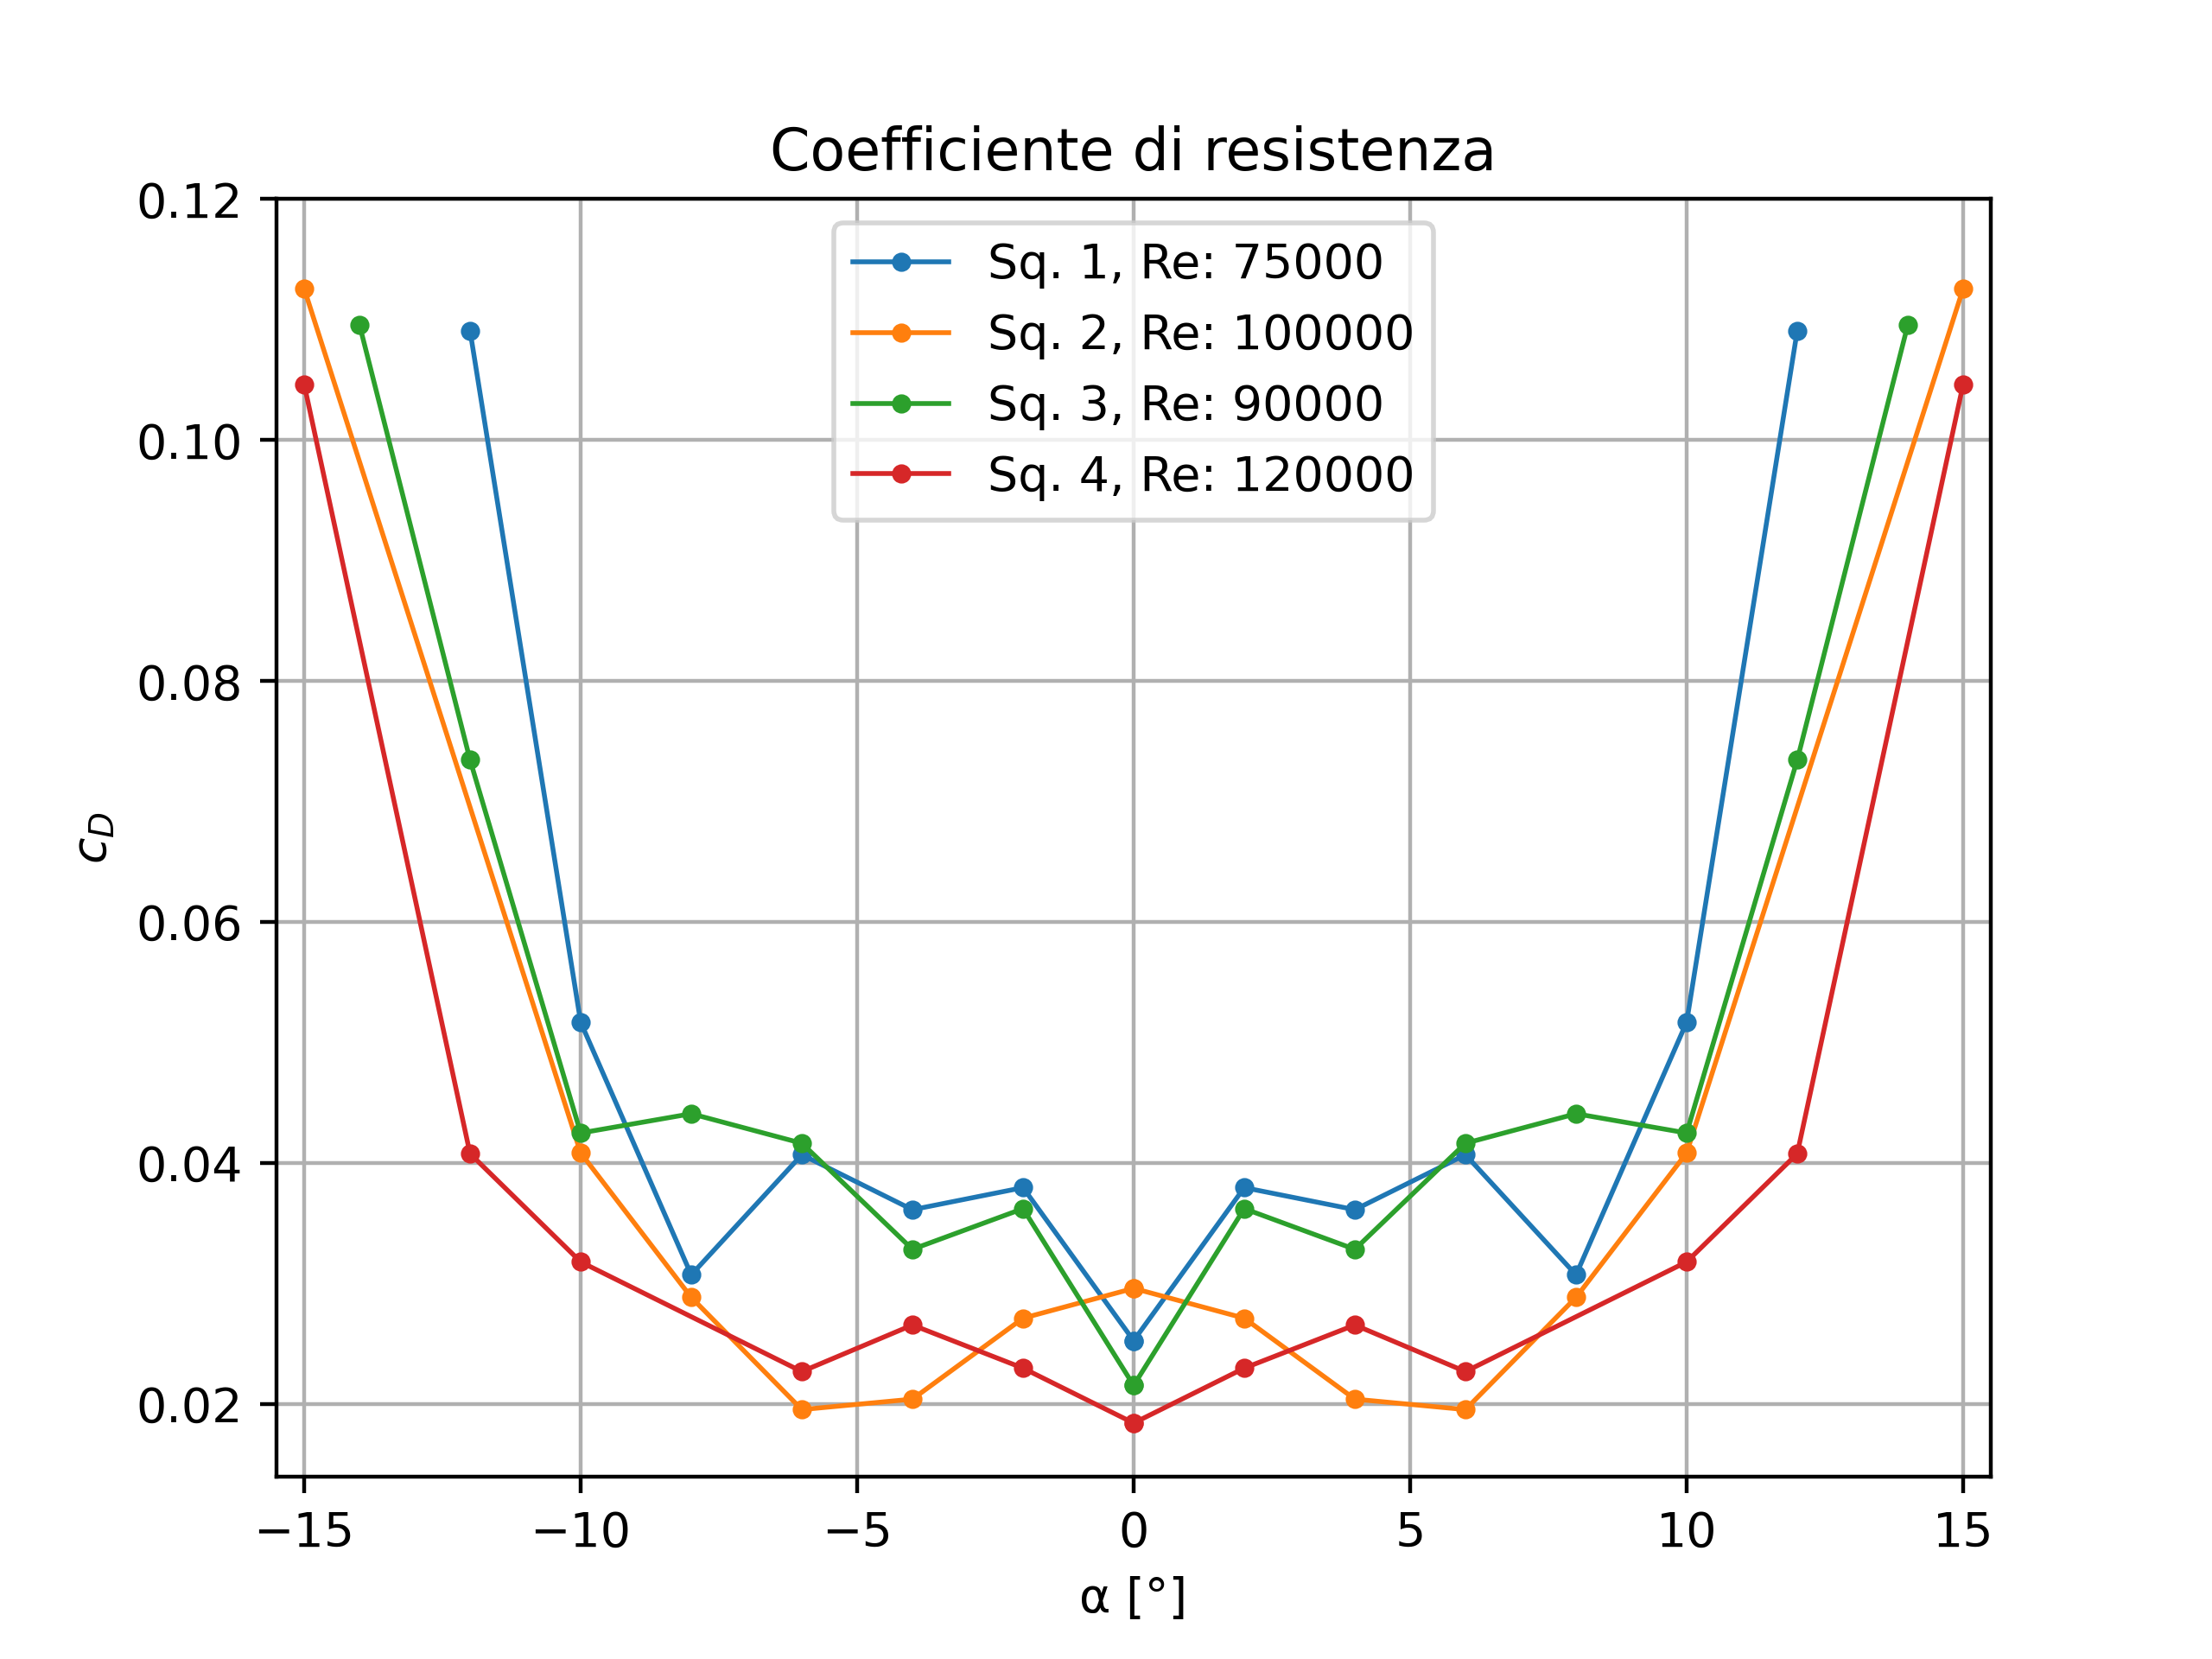
\includegraphics[width=.8\textwidth]{images/6/cd.png}
    \caption{Coefficiente di resistenza aerodinamica}
\end{figure}

\noindent Si osserva, come atteso dalla teoria, che la resistenza aumenti drasticamente in corrispondenza della condizione di stallo.\\\\
Si nota inoltre l'influenza del numero di Reynolds, le curve con un numero di Reynolds più basso risultano infatti più interne rispetto alle curve caratterizzate da un numero di Reynolds più alto.
\newpage
\subsubsection{Polare aerodinamica}
\noindent Utilizzando i valori del coefficiente di portanza in funzione dell'incidenza ricavati nell'attività precedente, è inoltre possibile diagrammare la polare aerodinamica del profilo, cioè la curva che mette in relazione il coefficiente di resistenza $c_D$ con il coefficiente di portanza $c_L$:
\begin{figure}[H]
    \centering
    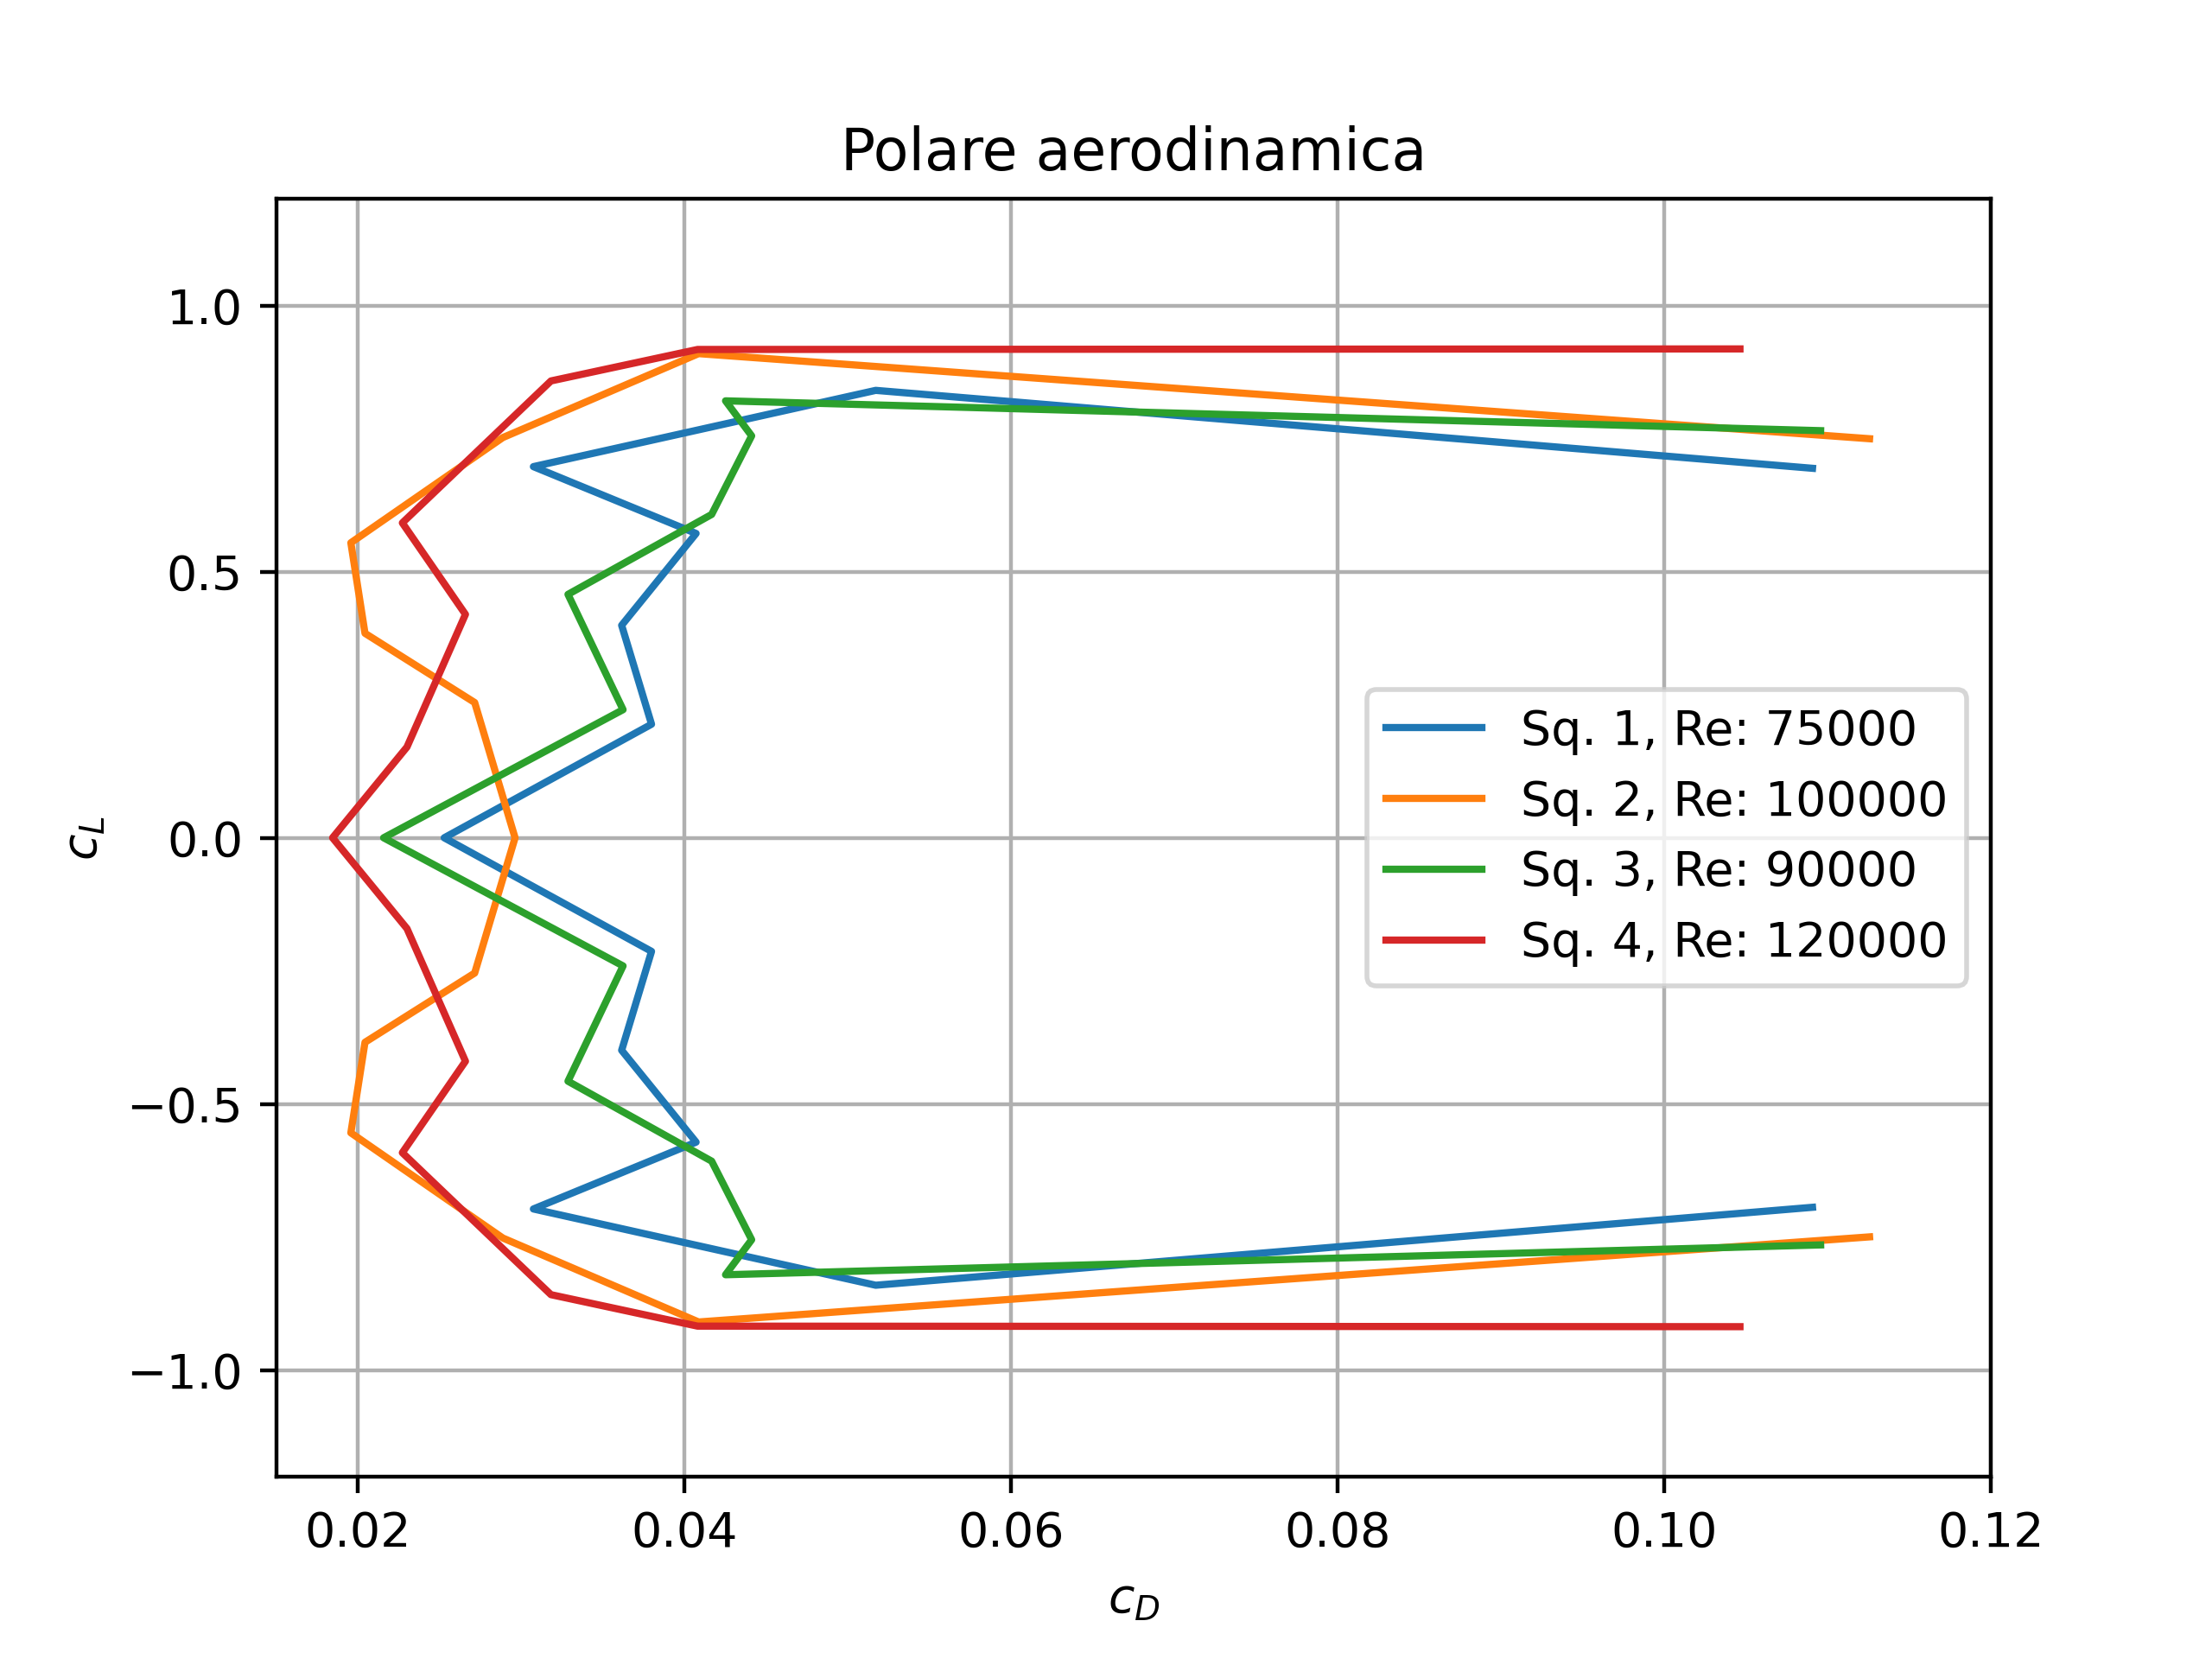
\includegraphics[width=.8\textwidth]{images/6/clvcd.png}
    \caption{Polare aerodinamica}
\end{figure}

\noindent Da questa immagine risulta evidente come in corrispondenza della condizione di stallo il coefficiente di portanza si riduce mentre il coefficiente di resistenza aumenta drasticamente.\\\\
Si osserva inoltre l'influenza del numero di Reynolds, le curve con un numero di Reynolds più basso risultano infatti più interne rispetto alle curve caratterizzate da un numero di Reynolds più alto.\\\\
Il numero di Reynolds sul coefficiente di resistenza ha un effetto benefico, con l'aumentare del numero di Reynolds infatti il profilo ritarda lo stallo e riduce leggermente la resistenza poiché lo strato limite turbolento rimane attaccato più a lungo dello strato limite laminare, che tende a separare appena incontra il gradiente di pressione avverso subito dopo il punto di massimo spessore del profilo.

\newpage
\subsection{Confronto con XFOIL}
Per validare i risultati sperimentali ottenuti, si eseguono delle analisi sul profilo alare NACA 0015 utilizzando il software gratuito XFOIL. Per numeri di Reynolds pari a 50000 e 100000, si ottiene la curva $c_D$-$\alpha$ illustrata nel seguente diagramma:
\begin{figure}[H]
    \centering
    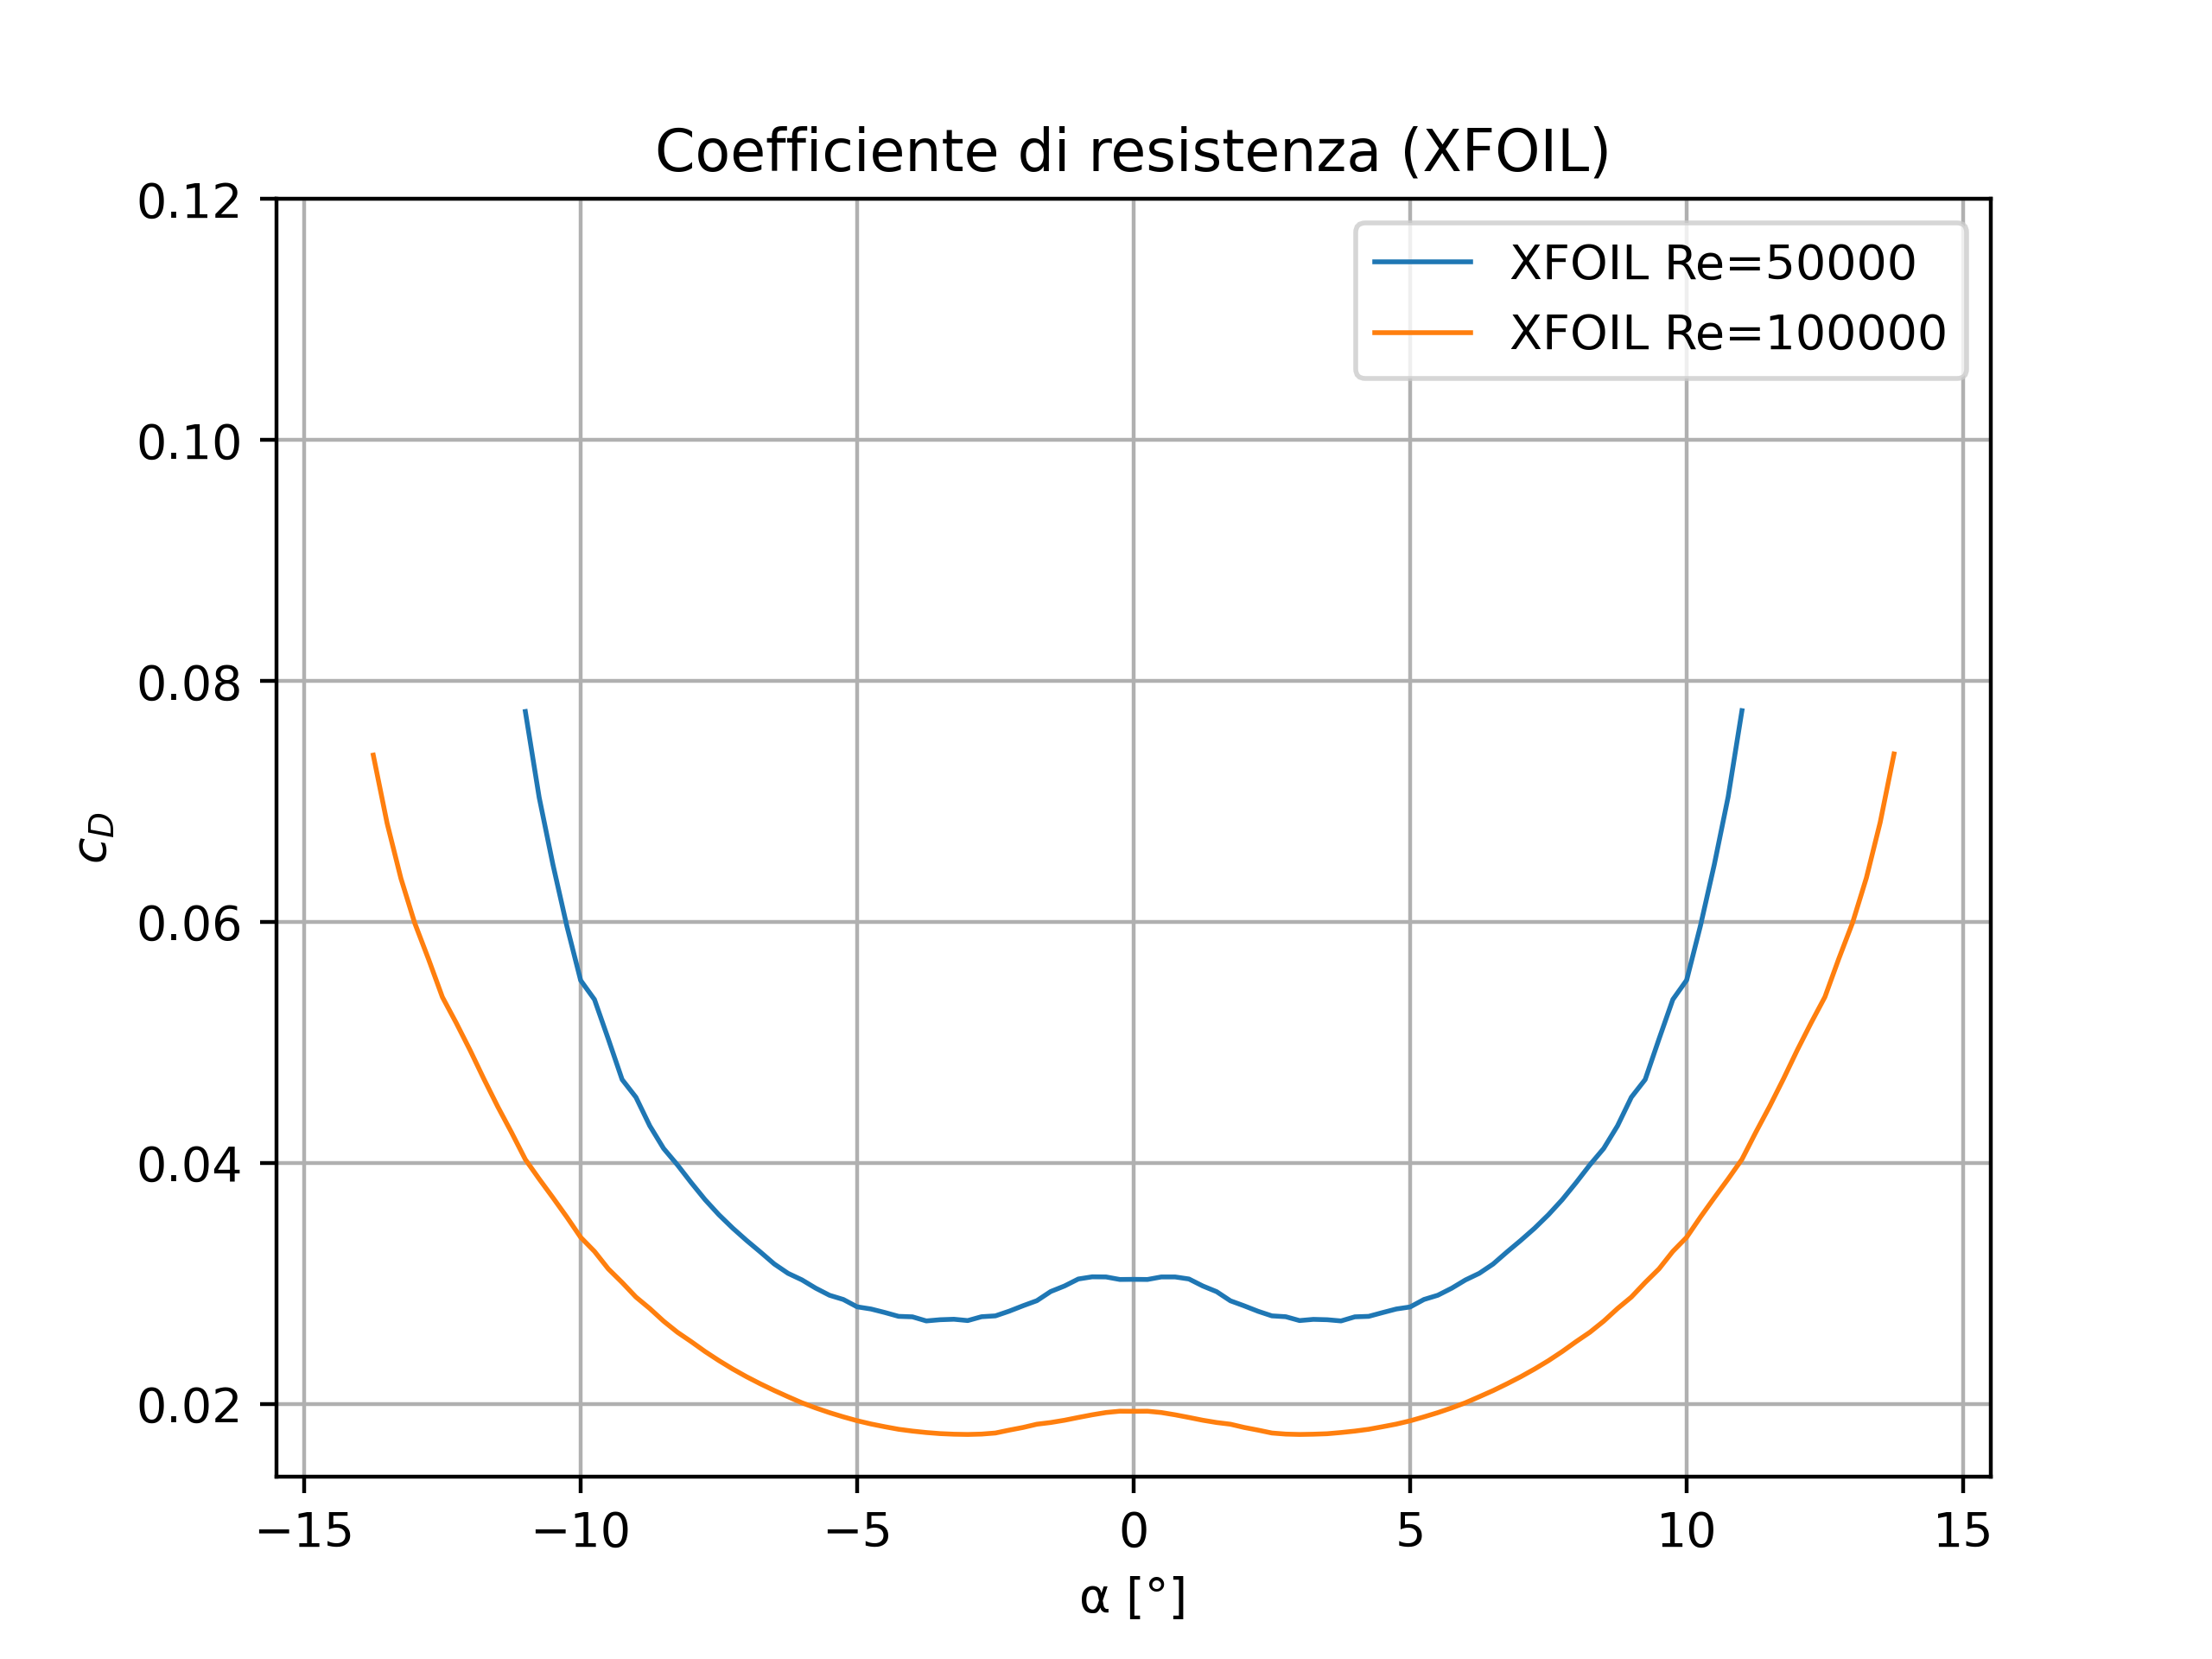
\includegraphics[width=.65\textwidth]{images/6/xfoil.png}
    \caption{Coefficiente di resistenza aerodinamica (XFOIL)}
\end{figure}
\noindent Si valuta inoltre la polare aerodinamica:
\begin{figure}[H]
    \centering
    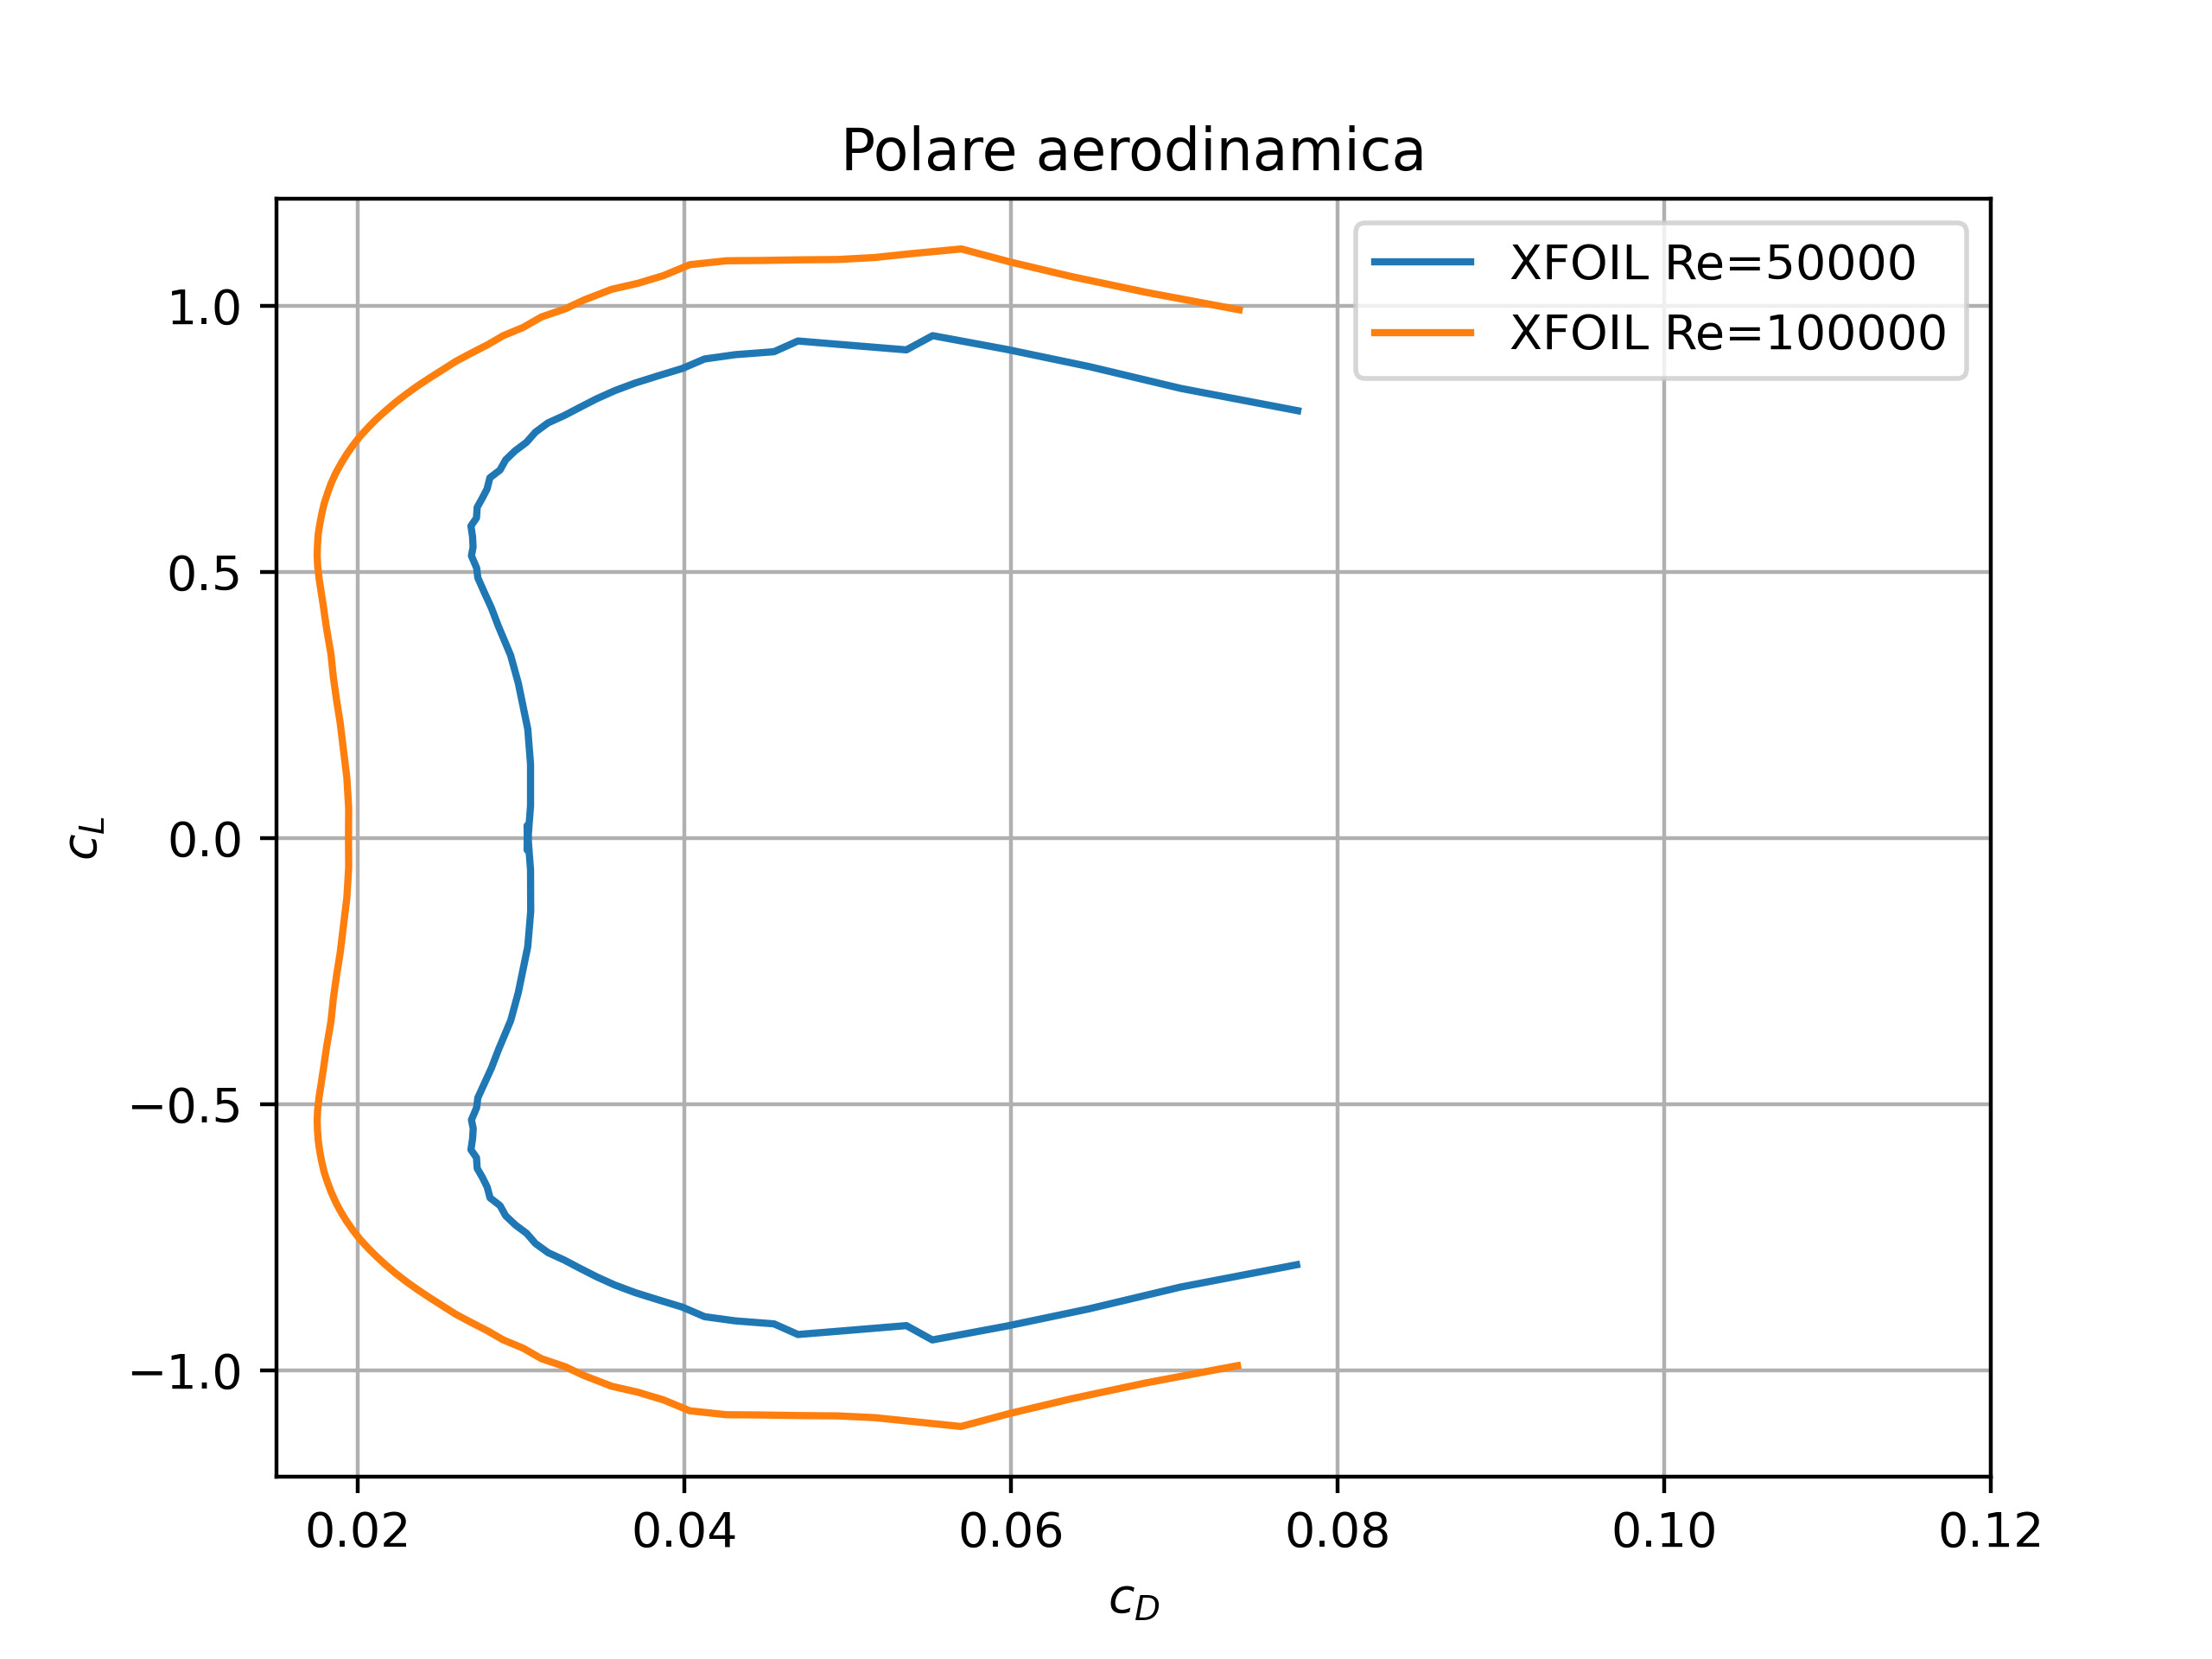
\includegraphics[width=.65\textwidth]{images/6/clvcdxfoil.png}
    \caption{Polare aerodinamica (XFOIL)}
\end{figure}

\noindent Si osserva come i risultati sperimentali corrispondono quasi perfettamente ad i risultati ottenuti utilizzando XFOIL.

